\section{Fears of What May Be, Erring Popes \& Councils}

\begin{wrapfigure}{rt}{.35\textwidth}
 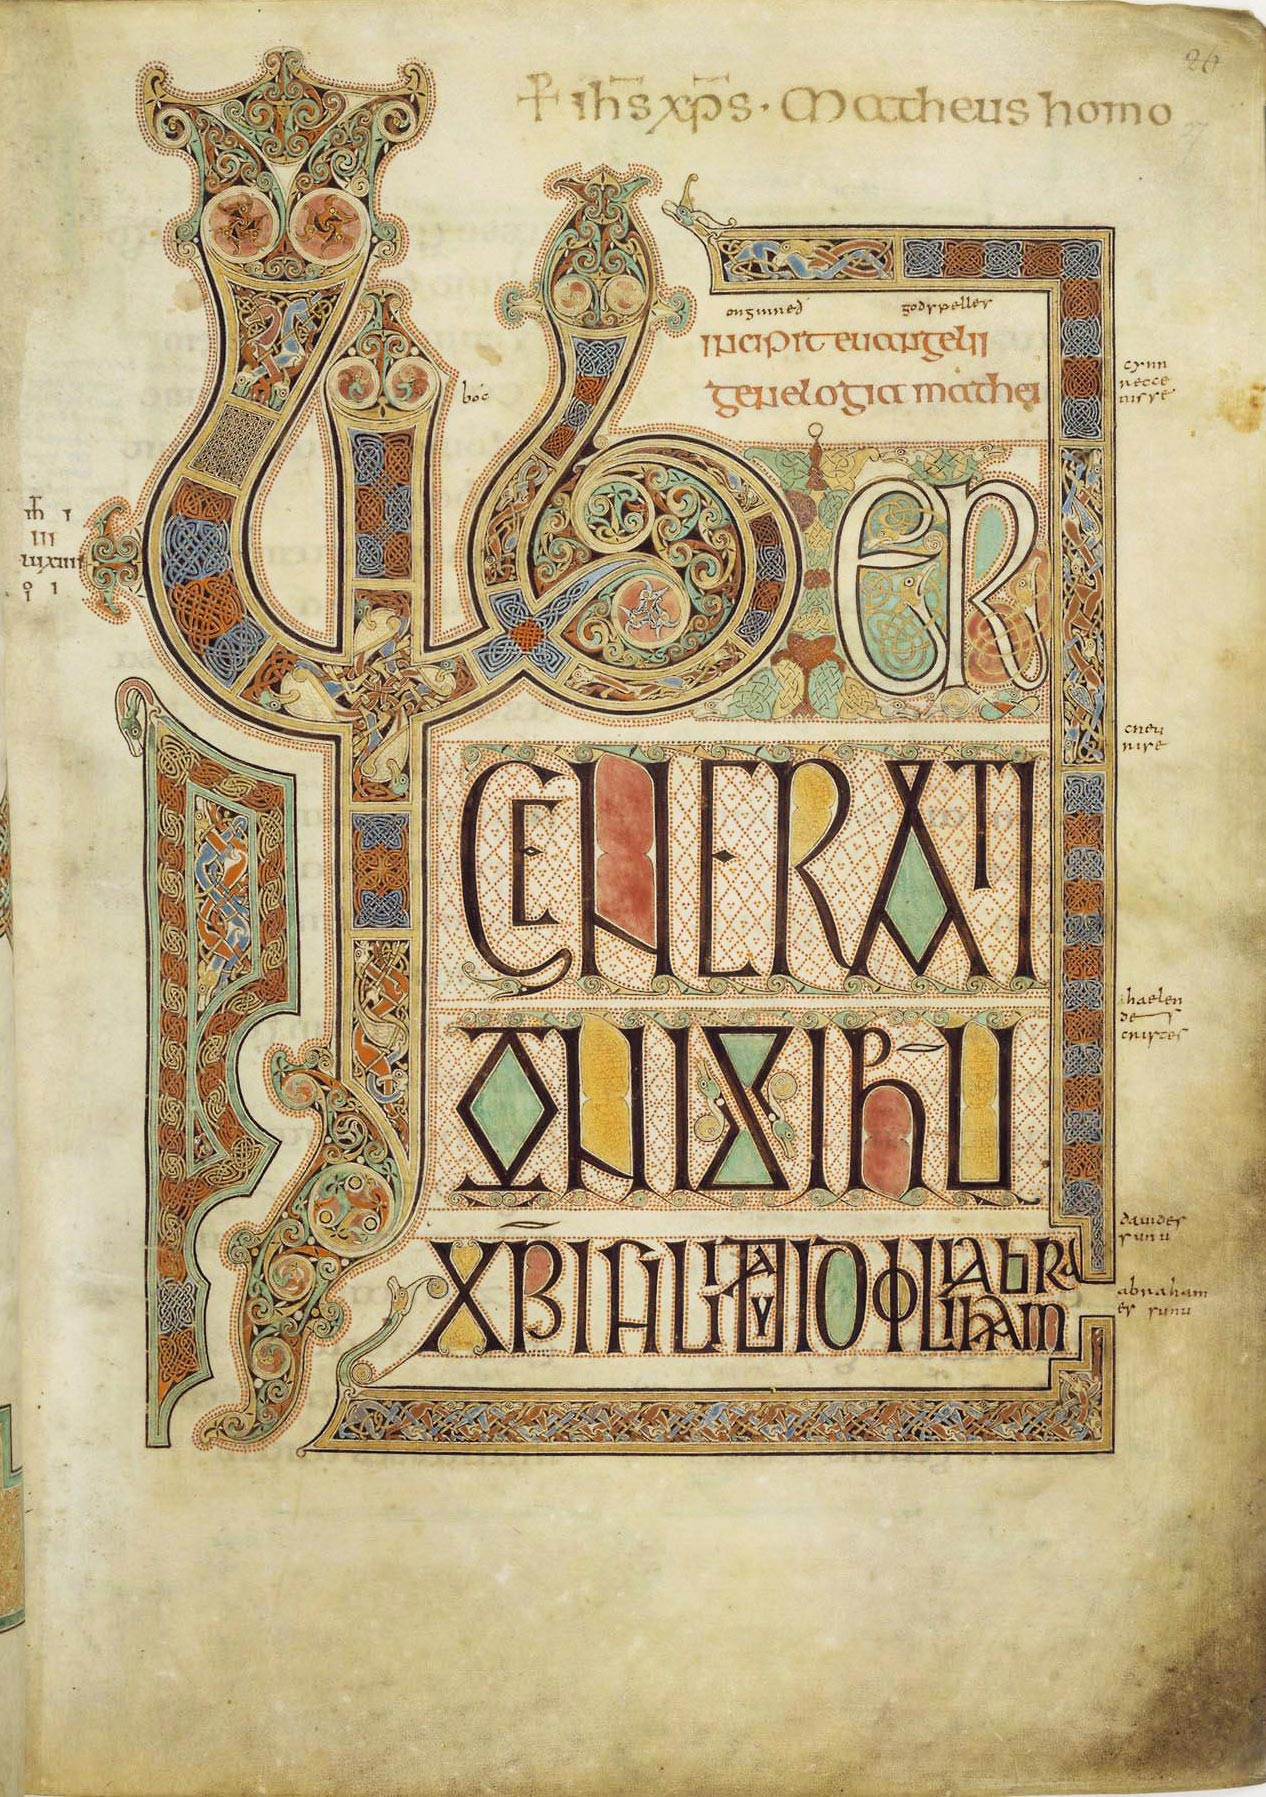
\includegraphics[scale=.09]{a20111224FearsofWhatMayBeErringPopesCouncils-img001.jpg} 
\end{wrapfigure}

\emph{Extra Ecclesiam non est salus: without (outside) the Church there is no salvation. }This was the motto of the Christian Church during the Medieval Era, and (supposedly) that which is objectionable in the Church today – the neo-pagans argue that the Church assimilated and reduced what it could not destroy.\emph{ This argument is actually true, but not in the sense which the neo-pagans intend it to be. }The Church did indeed enter a phase of development which represented a diminution, but it was not because it had combated paganism, but because it had decayed the patrimony which those same pagans had entrusted to it.


Specifically, the Church rejected the tripartite definition of man which had been handed to it by those who converted into the Church because they saw something worthy of merit which completed their aspiration. The Fourth Council of 869 AD (note that Constantine had long ago ``done his dastardly deed") repudiated a sophisticated, metaphysical view of man's nature in favor of something more exoteric and easy to understand.


\begin{quotex}
Though the old and new Testament teach that a man or woman has one rational and intellectual soul, and all the fathers and doctors of the church, who are spokesmen of God, express the same opinion, some have descended to such a depth of irreligion, through paying attention to the speculations of evil people, that they shamelessly teach as a dogma \emph{that a human being has two souls}, and keep trying to prove their heresy by irrational means using a wisdom that has been made foolishness.

Therefore this holy and universal synod is hastening to uproot this wicked theory now growing like some loathsome form of weed. Carrying in its hand the winnowing fork of truth, with the intention of consigning all the chaff to inextinguishable fire, and making clean the threshing floor of Christ, in ringing tones it declares \textbf{anathema} the inventors and perpetrators of such impiety and all those holding similar views; it also declares and promulgates that nobody at all should hold or preserve in any way the written teaching of the authors of this impiety. If however anyone presumes to act in a way contrary to this holy and great synod, let him be \textbf{anathema} and an outcast from the faith and way of life of Christians.\footnote{Source: \url{http://www.piar.hu/councils/ecum08.htm}}

\end{quotex}

The esotericism of the Church which had survived Justinian's codification was declared out of bounds. The time of this council was well after the ``Roman" phase of the Church had ended, after the chaos of the Dark Age invasions by Lombards, Franks, etc. The Roman Catholic Church (RCC) was essentially struggling to maintain what it could, both of the Greek connections \& the ancient Roman ones. John Romanides\footnote{\url{http://www.romanity.org/htm/rom.03.en.franks_romans_feudalism_and_doctrine.01.htm}} has some helpful articles detailing the unintended consequences of Charlemagne's adoption of Rome. Although he is incorrect to exaggerate the damage done from a proto-Greek perspective, he is certainly right to perceive that the chaos of the Western invasions did immense damage to all Roman institutions. \emph{Conditions in the West were so bad that Church fasts were lifted in order that populations might eat meat in order not to starve}. For the West, it was the Roman Church, or nothing – Chaos. It is unfair, then, to assume that perfect freedom of choice was exercised when the Church ``misplaced" or misunderstood its patrimony. Esoteric meaning can be lost in the best of times (just look around you); how, then, can we assume a deliberate error? Instead, one ought to look for what is best.

The case of Iceland\footnote{\url{http://www.pitt.edu/\~dash/njal100.html}} proves the point; one man's respected voice won a reprieve for paganism there, but only a private toleration – this man was actually a pagan priest. Additionally, the main proselytizing was done on the basis of ``trial by battle", a conflict in which (apparently) the archangel Michael came out over the berserkers, rune curses, and armies and storms of the pagan Gods.\emph{ And what was the price? Not to eat horsemeat, nor to expose the infants at birth to the elements!}

Note, also, that the conversion was done by royal decree \& blessed by a heathen seer who had converted :

\begin{quotex}
Shortly after Olaf Tryggvason became King of Norway he decreed that the old faith should be discarded and replaced with Christianity. His decree extended also to the islands of Shetland, Orkney, and Faroe.

When news of Norway's conversion reached Iceland, it was received by many with great anger. ``It is monstrous," they said, ``to forsake our ancient beliefs."

But Njal, a respected leader known for his ability to foresee the future, replied, ``I support the new faith. I believe that Christianity is a better religion than our old one. Those who accept it will be happy."

\end{quotex}
The rune magic which was supposedly lost was already very weak, just as Druidism had already been proscribed through battle and law by the Roman Empire. See, for instance, the account of the battle at the Isle of Anglesey\footnote{\url{http://www.philipcoppens.com/anglesey.html}}. Christianity actually preserved many remnants of paganism and gave them (arguably) a new life. This is not to minimize the bigotry of (for instance) Norman priests in England after the Conquest, but is merely to recognize that the policy of the Church towards paganism is not a simple matter of clear-cut answers. Surely, if paganism had been potent at that point, St. Boniface and others would not have been able to hew down sacred groves for firewood? When King Edwin converted based on the famous sermon with its analogy of a sparrow flying through the hall, from one door to the other, the instance\footnote{\url{http://markmeynell.wordpress.com/2010/09/10/king-edwin-of-northumberlands-conversion-and-the-sparrow-in-the-storm/}} proved that paganism had already lost the metaphysical knowledge of its own rituals.

Steiner\footnote{\url{http://www.bibliotecapleyades.net/biblianazar/ahriman04.htm}} and others offer a different account of what was occuring at the time, which has an attraction neo-paganism lacks – it is esoteric. It purports to be the revealing of the inner-ness; neo-paganism (on the other hand) seems to (often) an appeal to a neo-liberal conception of ultimate ``freedom of religion", rather than a cosmic account of history.

\begin{quotex}
Perhaps the most brilliant and influential proponent of this Arabian culture were the Caliph Haroun al Rashid and his associates, in the Eighth Century AD. This culture was, as indicated above, brilliant in a way, but was also anti-evolutionary in that it failed to appreciate the Christ-Impulse and was infected with the Sorat/Ahriman influence from Jundi Sabur. Around this time the cosmic Intelligence began to ``fall to earth", out of the rule of Michael and in the ``heads" of Men; the Pan-Intelligence becoming individualized, personal intelligence. This process was a preparation for what was to culminate after the dawn of the Consciousness Soul Epoch in the Fifteenth Century: that Men were to experience their thoughts as coming from out of themselves, as a personal intelligence in individual freedom. In 869 AD the fateful Eighth Ecumenical Council in Constantinople declared to be heretical the doctrine of ``trichotomy": that the Man is body, soul and spirit — thus effectively ``outlawing the spirit" in Western Christendom, and plunging West-European mankind ever more deeply into material experience. While this Council was happening on earth, in the soul/spirit world Haroun al Rashid and his associates, who had recently died, conferred with the individuality of Aristotle and associates: Alexander and the ``Aristotelians", together with the ``Platonists" and the Knights of Arthur's Round Table. In this meeting Aristotle and his associates resolved to bring to earth a renewed and Christianized wisdom suitable for the epoch of individualized intelligence of the Consciousness Soul, but al Rashid and his party remained opposed to this Christianization. Subsequently, on earth, the Arabian impulse was carried forward by philosophers such as Avicenna and Averroës, who upheld a decadent and retrogressive quasi-Aristotelianism, which denied human-spiritual individuality surviving death. And the Platonists descended to earthly incarnation, up through the Twelfth Century, as teachers of the Christianized Nature-wisdom of the School of Chartres. (This wisdom later inspired Bruno Latini, and consequently his pupil Dante.) In the Thirteenth Century the Aristotelians incarnated into the Dominican Order, wherein, with the help of the Platonists then in the spirit-world, they upheld the doctrine of human-individual intelligence and immortality, in the subtle conceptual thinking of the Scholastic ``Realists", as against the Arabian philosophers. The greatest of the Scholastics was Aristotle himself, incarnated as Thomas Aquinas, the proponent of the reality of Pan-Intelligence in the form of concepts — the ``universals" — and of the reality of human-individual experience of intelligence. — After the end of Medieval culture and the beginning of the Consciousness Soul Epoch, al Rashid himself incarnated as none other than Francis Bacon, the fountainhead of modern, Ahrimanic scientism. (Paradoxically, Bacon was inspired by a high Initiate, who also inspired Shakespeare, Jacob Boehme, and Jacob Balde. [Karmic Relationships, Vol. II] Again: evolution is not a simple, two-sided conflict between ``good" and ``evil" — in a way, a nominalistic-empirical science ``had to" enter cultural development.) Ahriman intends to make the now-earthly human intelligence entirely, overly individualized and personal, so that it degenerates into mere cleverness, driven by lower instincts and divorced from universal reality. But while Baconian science gained ground on earth, in the spirit/soul world the Platonists and Aristotelians convened in a ``school" under the leadership of Michael. 

\end{quotex}
No matter what one thinks of Steiner (and keep in mind Evola's definition of re-incarnation), this account is at least a ``mystery" account of the secret history of the world, rather than a Romanticization of an era which we are at least as completely detached from, collectively, as we are from the world of traditional Catholicism.  \textbf{Certainly, the prohibition of the Holy Spirit at that council would explain the submersion of the esoteric stream in the West, so that it had to re-enter the Western world via Tomberg, Solovyov, and others much later on.}

Without the restoration of the tripartite doctrine, the veredictum of history on the Church will risk becoming that of John Keat's\footnote{\url{http://www.mrbauld.com/keatsva.html}} on the clergy of his day:

\begin{quotex}
Axioms in philosophy are not axioms until they are proved upon our pulses: we read fine things but never feel them to the full until we have gone the same steps as the author. The Consecration was – not amusing — there were numbers of carriages, and his house crammed with Clergy – they sanctified the Chapel — and it being a wet day consecrated the burial ground through the vestry window. I begin to hate Parsons — they did not make me love them that day – when I saw them in their proper colours — A Parson is a Lamb in a drawing room and a lion in a Vestry. The notions of Society will not permit a Parson to give way to his temper in any shape – so he festers in himself – his features get a peculiar diabolical self sufficient iron stupid expression. He is continually acting. His mind is against every Man and every Mans mind is against him. He is an Hippocrite to the Believer and a Coward to the unbeliever – He must be either a Knave or an Ideot. And there is no Man so much to be pitied as an ideot parson. The Soldier who is cheated into an esprit du corps – by a red coat, a Band and Colours for the purpose of nothing – is not half so pitiable as the Parson who is lead absurdities – a poor necessary subaltern of the Church –

\end{quotex}
This sad state of Churchism as opposed to Christendom will come to pass, not because neo-paganism was correct in assuming the Church to be an alien usurper upon the Northern heritage, but rather, precisely because the Church failed to preserve a heritage given it by those very pagans who converted, and failed to have it restored by those pagans who picked up their mantle and immediately denounced the world their ancestors created. This is because they are dubious metaphysicians, and incline rather to a ``poetic" view of history; even the poets knew better than that:

\begin{quotex}
This is the very thing in which consists poetry; and if so it is not so fine a thing as philosophy-For the same reason that an eagle is not so fine a thing as a truth-Give me this credit-Do you not think I strive-to know myself? Give me this credit-and you will not think that on my own account I repeat Milton's lines\~{}

``How charming is divine Philosophy

Not harsh and crabbed as dull fools suppose

But musical as is Apollo's lute" 

\end{quotex}
Keats saw the errors of the Church, but used poetry to intuit the ancient doctrines of ``the vale of soul-making" \& the ``house of many mansions" — it's a pity he couldn't have read Guenon on states of being. It would be easy to pillory the Church (and I agree with Keat's analysis of many parsons), but it is the harder (and more productive) to abandon invective, and to pursue the ``great work" of following the Spirit.

Tomberg puts it this way:

\begin{quotex}
Dear Unknown Friend, do not interpret what I am saying in the sense that I am opposed or even hostile to the above-mentioned societies, fraternities, and movements of a spiritual and initiatory nature, nor in the sense that I am accusing them of an anti-Christian attitude. Do not attribute me with a lack of respect for the mahatmas and gurus of India. It is a matter here only of the purely psychological tendency (that I have been able to observe something of everywhere) which prefers the ideal of the superman to the ideal of the Son of Man. 

\end{quotex}
Tomberg goes on to add (this is the sixth chapter of MotT, the Charioteer) that the tendency is everywhere resisted in these organizations, that tendency to the three temptations of mania, inflation, and megalomania. But he insists that it is most effectively combated within the doctrine of the Church, which teaches that ``the Lord" safeguards the sanity \& humility of the initiate.

Isn't this what the West has always aspired to? The mutual recognition of truth under the umbrella of Truth? What is to prevent the practice of this, upon either side of the Roman wall?



\flrightit{Posted on 2011-12-24 by Logres }

\begin{center}* * *\end{center}

\begin{footnotesize}\begin{sffamily}



\texttt{Charlotte Cowell on 2011-12-25 at 13:27 said: }

A few thoughts sprang to mind when I read this. Firstly (in passing, really), I had never heard of this `twin soul' heresy or that it was so controversial. I think I need more info about what is what – are literally two souls what is meant or is it a soul and spirit issue?

Secondly, I agree Steiner can shed light on very difficult parts of the path, although I do not necessarily share his express view of reincarnation. Reading this made me wonder whether viewing reincarnation as a form of channelling might help solve the problem (making it more a question of terms)?

I think the Chariot card may be number 7 but either way I was put in mind of the Phaedron Charioteer and the twin horses of the soul – maybe some are getting the soul confused with its horses? Just an idea, here's an extract by the way: \url{http://alchemical-weddings.com/alchemical-weddings/the-phaedrus-charioteer}

I just found something from The Chariot card on my blog, the philosophy of a lunatic, which always amuses me:

\url{http://alchemical-weddings.com/alchemical-weddings/philosophy-of-a-lunatic}

I tarried not to tie my sandal shoe, but haste, post haste, through air my winged chariot flew (Aeschylus, Prometheus Bound)


\hfill

\texttt{logres on 2011-12-25 at 17:01 said: }

Charlotte, I've had that thought, too – perhaps there is an element (the one atom that we never replace, according to Max Heindel) which is imperishable and the seat of immortality in the soul which corresponds to Evolan individuality, but (then) the ``truth of reincarnation" would simply be the experience of having a supra-personal + sub-personal ``flame" of being passed on which records an imprint of the seat of immortality (in worship of the previous bearer). ``Channeling" could work that way. Incidentally, I need to ask you a question about waking up in dreams. I've had a lot of dreams where I am doing things with my hands, but can't remember to ask myself why.


\hfill

\texttt{Charlotte Cowell on 2011-12-25 at 17:14 said: }

well the way I see it we all have a spark of the divine with us, and the way of return is analogous to the Kabablistic process of `raising the sparks', by which all souls/spirits return to the divine source. But I can see how the idea of it being a flame lends itself to the notion of passing on the torch. In the case of a great light like St Augustine, you might reasonably expect many torches of inspiration, wisdom, etc to be lit as a result of his endeavours, although you wouldn't necessarily say he's reincarnating over and again in students. It just suddenly struck me as I was reading that part of the post about Steiner that Thomas Aquinas might well have ended up `channelling' Augustine if he studied his works in great depth and fully absorbed them into himself. What intrigues me more is how Steiner saw himself. Clearly Steiner was clairvoyant but clairvoyant vision is so rich in symbolism and has so many layers that perhaps it's all just a matter of interpretation. Certainly Steiner doesn't go out of his way to spoon feed or make things especially simple for his readers….often he's very challenging, I think he's the sort of teacher that can be wrong so the student can reach a correct answer. Mystery teaching isn't `easy' at the best of times, let alone from beyond the grave. 

What do your hands look like, what kinds of things are they doing?


\hfill

\texttt{Charlotte Cowell on 2011-12-25 at 17:17 said: }

or maybe it was Aristotle, I can't remember, point still applies tho…didn't Aristotle use ellipses?!


\hfill

\texttt{logres on 2011-12-25 at 22:26 said: }

Typing, right now! Ring on finger, left hand, wedding. I've tried to memorize the vein patterns, or note scars. Lately, have been trying to be ``aware" of them at odd intervals in the day. Realized I usually look at object ``in hand", not at them.


\hfill

\texttt{Charlotte Cowell on 2011-12-26 at 09:38 said: }

when I saw my hands in a dream I was taken aback by how they looked, it wasn't like looking at my physical body


\hfill

\texttt{logres on 2011-12-26 at 12:26 said: }

I can't remember to look, in the dream.


\hfill

\texttt{Caleb Cooper on 2011-12-26 at 16:07 said: }

You're lucky that you saw something so beautiful Charlotte. The night after you first mentioned the practice I decided to look at my hands while dreaming. They took on an unstable character, the fingers fusing together and separating, their size distorting around the edge of my awareness, in a reminder of the ugliness of my unintegrated soul. 

It was a strange experience. Like my awareness was trying to catch and hold the hands in a stable form, but it was too slow, traveling through an unpleasant invisible molasses, and right when it might catch them it hit a thicker patch a few inches from the hands which it would slide off, the hands distorting with the slipped awareness. 

Had a more pleasant experience looking at my hands in a dream tonight. I didn't see the luminous body or anything, but they appeared quite beautiful, probably because I was holding one of my soul fragments in my palms and healing it, so there would have been a very high stable frequency going through them at the time. But when I'm not elevated above my base state, yeah, pretty ugly. I should experiment with focusing the awareness on other parts of my body in the dreaming so I can see just how fucked up my soul is there as well:)


\hfill

\texttt{Boreas on 2011-12-26 at 16:36 said: }

This conversation brought to my mind a music video that reminds me about dreaming, dreams and the astral world in general – and about hands. I don't if the symbology in the video is some kind of a ``hint" to dream workers, but even if it's not, it's still quite fitting: \url{http://www.youtube.com/watch?v=0rs\_NRyNs4o}

(You need to look it through to understand my point.)

Years ago, when I tried to awake in my dreams and did practices to accomplish this, one of the basic practices was to serach for my hands in dreams and to memorize this while in awake in order it to become a habit while sleeping and seeing dreams. I never got any amazing results this way, but I think and have heard that many have.

Hands, like eyes, are the mirror of the soul and its constituting principles, and the alchemical planetary correspondences and the chakric correspondences can tell alot about many things; I always get smaller or bigger cuts and wounds in my fingers or palms if there's something that I've done or said wrong – the size of the ``reflection" (=wound) symbolising the level of the mistake, and the place of the wound the corresponding principle to look up to.


\hfill

\texttt{Boreas on 2011-12-26 at 17:19 said: }

Charlotte said: ``I think I need more info about what is what – are literally two souls what is meant or is it a soul and spirit issue?"

I don't have the exact information, but it might be a major mis-interpretation of the concepts of the animal soul and the rational soul, and the corresponding teachings in different traditions (kabbalah tree of life, germanic / nordic paganism etc.)

\texttt{Logres said: ``What is to prevent the practice of this, upon either side of the Roman wall?"}

The same as always: human stupidity and selfishness combined with myopic worldly goals. But lets not lose our hopes that at least those ``who are still gathered at the Vulture's peak" (or listening the ones who are gathered there!) understand and learn how to reconciliate their own paths and personal truths in the light of the greater unity.


\hfill

\texttt{Charlotte Cowell on 2011-12-26 at 17:29 said: }

Caleb, they did not really look beautiful more strange – translucent and kind of grey, I was quite weirded out by it, as I was when I saw my astral self in a mirror once, that freaked me out a bit


\hfill

\texttt{Charlotte Cowell on 2011-12-26 at 17:31 said: }

Boreas, the hands thing is the method taught my Don Juan to Carlos in the Carlos Castaneda novels – it is not so much the fact that one is looking at the hands that makes one conscious, but the fact one remembers to do something – looking at the feet would presumably be as efficacious, although there is something about hands as you point out….


\hfill

\texttt{Boreas on 2011-12-26 at 17:39 said: }

From the link to the article `Iceland Accepts Christianity' this caught my eye…

``In the meantime, the chieftains meeting at the Althing outlawed Hjalti Skeggjason for having blasphemed Freyja and Odin by calling them a bitch and a dog in his poem."

…and sent streams of joy through my soul, haha.

But seriously speaking, it also reminds one about the fact how easily the old truths are forgotten and denied in the frenzy of `conversion' (apparent or real), for better or for worse (usually the first option), and how easily the baby is thrown away with the bath-water.

The Gods never left the old heathens, the heathens forgot and abandoned them to a great extent, and they also failed to renew their traditions in the way that they would have provided them the needed spiritual and cultural nourishment. Now the same fact applies greatly to both neo-pagans and to (neo-)christians, while at the same time on the outer world fundamentalism, atheism and nihilism abound. This is why a synthesis in the light of universal esoteric knowledge is so greatly needed in our time and in the following age.


\hfill

\texttt{Boreas on 2011-12-26 at 17:40 said: }

Argh, a slip!

``usually the first option" –{\textgreater} usually the \_second\_ option


\hfill

\texttt{Boreas on 2011-12-26 at 18:00 said: }

OK. Based on this I take it could be an old shamanistic practice, since Castaneda fused (and confused) many teachings on his writings. I don't think it's the same – or a mere practical thing – if you look upon the hands or upon the feet. The right HAND path \& left HAND path and so on…!

However, here's one animation link for the chakric correspondences:

\url{http://www.iloveulove.com/images/ss\_kundalini\%20anim.gif}

And a picture for the planetary correspondences:

\url{http://ccrsdodona.org/images/1977\_sag\_palm1.gif}

The color scales and the planetary symbols co-incide and relate to each other quite well, yet I'd say that the either the Sol symbol in the planets or the golden color upon the chakric finger correspondences are mis-placed.

``The science of hand-reading, strange as this may seem to those who have no notion of such things, is, in its Islamic form, directly related to the science of the divine names: the arrangement of the principal lines of the left hand trace out the number 81, and those of the right 18, giving a total of 99, which is the number of the names attributed to Allah (sifatiyyah). As for the name Allah itself, it is formed by the fingers in the following way: the little finger corresponds to the alif, the ring finger to the first lam, the middle and index fingers to the second lam, which is double, and the thumb to the ha (as regularly drawn in its `open' form): and here lies the principal reason for the widespread use of the hand as a symbol in all Islamic countries. From this we may understand the meaning of the verse in the book of Job: `He seals up the hand of every man, that all men may know his work': and it may be added that this is not unrelated to the essential role of the hand in the rites of benediction and consecration…"

– René Guénon, Insights into Islamic Esoterism and Taoism'


\hfill

\texttt{logres on 2011-12-27 at 00:54 said: }

Thinking about this today (I appreciate all the helpful comments, maybe this will help me) – the hands are the active part of the soul. When the mind is SURE and stable, you can concentrate on doing with the hands. Perhaps, in a dream, the hands can only become visible when the mind has reached a certain stability. Also, you may be reaching to DO something in a place that you are not yet ready to act – hence, the wavy hands. Heindel teaches that in past epochs, as the vehicle of the body was prepared, the spirits were attached, but not fully incarnated – they then experienced through the body, but not fully as we do. Something similar is going on with the hands in dreams. A fully awake person would have dream hands that were beautiful. Or at least not streaming off somewhere. They may be connected to another place, even inside the dream. That is backward, from the hands, down, rather than from the feet, up.


\hfill

\texttt{Charlotte Cowell on 2011-12-27 at 08:08 said: }

well the real and/or imaginary Don Juan was eminently practical, and when he revealed the purpose of the exercise to Carlos he said that it was the consistent effort involved with trying to see the hands (or whatever) that made the unconscious self absorb the practice so completely that at some stage one will inevitably see the hands. It's interesting what the Sufis/Guenon said about hands and one intuitively feels there's something significant about this part of the body having been chosen, but in the `Don Juan school' they're not relevant in this way. His goal was simply to heighten perception. I've never heard of the hands streaming off or away before, or any other part of the body, that sounds like a dream to me. As far as I'm aware the astral self doesn't dissemble in this way and (in my experience) people generally appear as their most beautiful possible selves in that state, it can be quite intersting to see how the otherwise secret character and beauty of an individual manifests, especially with respect to the light in their eyes.


\hfill

\texttt{logres on 2011-12-27 at 13:48 said: }

It was just a speculation – I've heard the hands look wispy or wavy, suggesting a movement to another plane. As I say, I've yet to accomplish it – my dreams for now are rather jumbled, although changing. Happy twelve days, to all!


\hfill

\texttt{Caleb Cooper on 2012-01-01 at 16:51 said: }

On the original post, I think Rome's position is a little more nuanced, and if I understand correctly, compatible with Traditional teachings on the tripartite nature. 

At my last RCIA class before Christmas break, there was a reading from St. Paul in which he used Spirit distinct from soul, giving me the opening to ask the Deacon what the Catholic distinction between them was. The Deacon's explanation was that God has breathed a Spirit into all men, and this Spirit is the Holy Spirit. I was quite pleased to hear this, as it seems essentially in agreement with Tradition, that the Spirit in man is a fragment of God, which also contains the entirety of God (like a hologram).

I'm not familiar enough with Church history to speak with authority, but what Constantinople IV may have been objecting to was the demoting of Spirit in man to the level of a soul, in which case they were actually defending the tripartite view of body/soul/spirit against body/lower soul/higher soul, which cuts man off from the higher spiritual vistas.


\hfill

\texttt{logres on 2012-01-02 at 01:00 said: }

Caleb, that's actually a very astute comment, \& Cologero privately pointed out the same thing, so the Council's ``error" may have been more one of context (ie., in the process, losing the instinctual point and definite dogma being incidentally touched upon by way of clarification) than of intent. A study on the dearth of tripartism in the Church might prove interesting and turn up more facts. This was meant to be introductory, \& I obviously have a lot more to learn on the subject. However, the lack of clarification or context is troubling.


\hfill

\texttt{logres on 2012-01-02 at 01:08 said: }

Boreas, the blaspheming poet got what he deserved, so it's comforting that there is some justice in the world. You may be interested in \url{http://www.sacredscience.com/archive/GodwinArcheometer.htm}, although you sound like you've already been over this ground.


\hfill

\texttt{Dimitri on 2023-03-08 at 12:51 said: }

Actually, I'd like to issue a correction to this article. I did some digging on the point of the Fourth Council of Constantinople (the Catholic one) because I found the language of Canon 11 suspicious, in that it didn't seem to be condemning a tripartite view of man; after all, why would it condemn the idea that man has ``two souls" (which is not the tripartite view), rather than both a soul (anima) and a spirit (spiritus), if they have two separate words for both in Latin? As it turns out, it was doing no such thing:

``The eleventh canon anathematizes the doctrine that a human being has two souls. This refers to a doctrine promoted by Photius, that each man has two souls, one that is liable to error and another that is immune to error. Photius himself did not believe this doctrine, but gave arguments in its favor in order to prove that theologians could not afford to ignore philosophy. Many people took these arguments in earnest and believed the doctrine, requiring its repudiation here." (Commentary on the Fourth Council of Constantinople, \url{https://www.arcaneknowledge.org/catholic/councils/comment08.htm})

Upon digging into the matter further, I found corroboration for this when I looked into what Photios the Great was attempting to do by putting forth this teaching:

``In a feud with Patriarch Ignatios, Photios invented a fanciful theory that people have two souls, for the sole purpose of tricking Ignatios into embarrassing himself by being seen to take it seriously, whereupon Photius withdrew his proposal and admitted he had not been serious."

Historical context is important, folks!


\hfill


\end{sffamily}\end{footnotesize}
